%
\section{Source code documentation}
\label{sec:source-code-docum}
Source code documentation is critical for software maintenance, specially on
large developments teams. As software applications grow in size and evolve
several modifications from base source code arise, possible with several
branches to implement different features or correct bugs. A good practice that
helps to reduce the complexity burden when interfacing and maintaining such
systems is to document the source code, making it readable and easily understood
by other people.

Source code documentation aims to describe how the code works instead of what it
does, and it is useful for the following
reasons~\cite{sourceCodeDocBestPractices}:
\begin{item-c}
\item \emph{Knowledge transfer}: not all code is equally obvious. There might be
  some complex algorithms or custom workarounds that are not clear enough for
  other developers.
\item \emph{Troubleshooting}: if there are any problems with the product after
  it's released, having proper documentation can speed up the resolution
  time. Finding out product details and architecture specifics is a
  time-consuming task, which results in the additional costs.
\item \emph{Integration}: product documentation
 describes dependencies between system modules and third-party tools. Thus, it
 may be needed for integration purposes.
\item \emph{Code style enforcement}: the source code documentation tools
  requires specific comment syntax, which forces the developer to follow a
  strict code style. Having a code style standard is specially useful on large
  project teams.
\end{item-c}

There are some key ideas to write good documentation~\cite{sourceCodeDocBestPractices}:
\begin{item-c}
\item  
\emph{Simple and concise}. Follow the DRY (Don't Repeat Yourself)
principle. Use comments to explain something that requires detailed information.
\item
  \emph{Up to date at all times}: the code should be documented when it's being
  written or modified.
\item
  \emph{Document any changes to the code}. Documenting new features or add-ons is pretty obvious. However,
 you should also document deprecated features, capturing any change in the
 product.
\item
 \emph{Simple language and proper formatting}: Code documents are typically written in English so that any
 developer could read the comments, regardless of their native language. The best practices for
 documentation writing require using the Imperative mood, Present tenses, preferably active voice, and
 second person.
\end{item-c}

There are several automatic source code documentation tools, typically
language-specific, namely~\cite{sourceCodeDocBestPractices}:
\begin{item-c}
\item \emph{\texttt{Doxygen}}: C, C++, C\#, Java, Objective-C, PHP, Python
\item \emph{\texttt{GhostDoc}}: C\#, Visual Basic, C++, JavaScript
\item \emph{\texttt{Javadoc}}: Java only
\item \emph{\texttt{Docurium} or \emph{YARD}}: Ruby
\item \emph{\texttt{jsdoc}}: Javascript
\item \emph{\texttt{Sphinx}}: Python, C/C++, Ruby, etc.
\end{item-c}

\subsection{Doxygen}
\label{sec:doxygen}
Doxygen is the de facto standard tool for generating documentation from
annotated C++ sources, but it also supports other popular programming languages
such as C, Objective-C, C\#, PHP, Java, Python, IDL (Corba, Microsoft, and
UNO/OpenOffice flavors), Fortran, VHDL and to some extent D.
Doxygen is highly portable, running on MacOS, Linux and Windows platforms~\cite{doxygenIndex}.

Doxygen supports the user in two ways~\cite{doxygenIndex}:
\begin{enum-c}
\item \emph{Flexibility in documentation generation}:
  It can generate an on-line documentation browser (in HTML) and/or an
  off-line reference manual (in \texttt{LaTeX}) from a set of documented source
  files. There is also support for generating output in RTF (MS-Word),
  PostScript, hyperlinked PDF, compressed HTML, and Unix man pages. The
  documentation is extracted directly from the sources, which makes it much
  easier to keep the documentation consistent with the source code.
\item \emph{Assistance in reverse engineering \gls{sw}}:
  You can configure doxygen to extract the code structure from undocumented
  source files. This is very useful to quickly find your way in large source
  distributions. Doxygen can also visualize the relations between the various
  elements by means of include dependency graphs, inheritance diagrams, and
  collaboration diagrams, which are all generated automatically.
\end{enum-c}

\subsubsection{Documenting the code}
\label{sec:documenting-code}
Doxygen uses special comment blocks, i.e., comment blocks with some
additional markings to identify source code annotations for the
documentation~\cite{doxygenDocBlocks}. As aforementioned, Doxygen supports several programming
languages, but here one focus only on C-like languages, specifically \texttt{C}
and \texttt{C++}.

For each entity in the code there are two (or in some cases three) types of descriptions, which together form
the documentation for that entity, namely~\cite{doxygenDocBlocks}:
\begin{enum-c}
\item \emph{Brief description}: short one-liner, briefly documenting the
  following block. It is optional.
\item \emph{Detailed description}: provides more detailed documentation about
  the following block. It is optional.
\item \emph{Body description}:
for methods and functions there is also a third type of description, consists of
the concatenation of all comment blocks found within the body of the method or
function.
\end{enum-c}

There are several ways to mark a comment block as a detailed description:
\begin{enum-c}
\item \emph{\texttt{Javadoc} style}: 
  consists of a C-style comment block starting with two \texttt{*}'s, as follows:
\lstinputlisting[
language={c},
firstline=43, lastline=45,%
caption={},
% label=lst:makefile-example,
style=customc]{./listing/doxygen_example.h}
%\vspace{-.8em}
\item \emph{\texttt{Qt} style}: add an exclamation mark (!) after the opening of
  a C-style comment block, as follows:
\lstinputlisting[
language={c},
firstline=47, lastline=49,%
caption={},
% label=lst:makefile-example,
style=customc]{./listing/doxygen_example.h}
%\vspace{-.8em}
\item \emph{slash style}: use a block of at least two C++ comment lines, where
  each line starts with an additional slash or an exclamation mark, as follows:
\lstinputlisting[
language={c},
firstline=51, lastline=53,%
caption={},
% label=lst:makefile-example,
style=customc]{./listing/doxygen_example.h}
\vspace{-.8em}  
\end{enum-c}

The style adopted by the authors is the \texttt{Javadoc}. Besides comment
blocks, annotations can be used at other levels:
\begin{item-c}
\item \emph{inline}: used to describe parameters, class members, and structure
  and enumeration fields.
\lstinputlisting[
language={c},
firstline=65, lastline=65,%
caption={},
% label=lst:makefile-example,
style=customc]{./listing/doxygen_example.c}
\vspace{-.8em}  
\item \emph{file}: used to describe modules or classes. The tags \texttt{@file},
  \texttt{@author} and \texttt{@date} are used to identify the file name, the
  author and the creation date; the tag \texttt{@brief} provides a brief
  description about the file and in the last lines is the detailed description.
\lstinputlisting[
language={c},
firstline=1, lastline=11,%
caption={},
% label=lst:makefile-example,
style=customc]{./listing/doxygen_example.h}
\end{item-c}

Listing~\ref{lst:doxygen-example-h} illustrates an example of a documented C
header file using Doxygen in the Javadoc style. Lines 1 through 11 document the
header file, explaining its purpose and the available public interface. Lines
16-19 document the opaque pointer to a \texttt{struct App\_T}. Lines 22-39
document the public interface of the module --- \texttt{App\_init} and
\texttt{App\_exec}. Specifically, considering the latter, it showcases \emph{how
  to document functions}:
\begin{item-c}
\item \emph{\texttt{@brief}}: briefly describing the function's purpose.
\item \emph{\texttt{@param}}: describing all parameters and its prerequisites,
  in this case, \texttt{app}.
\item \emph{\texttt{@return}}: identifying the return value of the function.
\item \emph{Detailed description}: providing further details about the
  function's operation.
\end{item-c}
%
\lstinputlisting[
language={c},
firstline=1, lastline=41,%
caption={Example of a documented C header file using Doxygen --- Javadoc style},
label=lst:doxygen-example-h,
style=customc]{./listing/doxygen_example.h}


Listing~\ref{lst:doxygen-example-c} illustrates an example of a documented C
implementation file using Doxygen in the Javadoc style. As a recommendation,
public interfaces should be documented in the header file and the private
implementation details in the implementation file. Once again, the file is
documented; inline comments are used for \texttt{\#define}'s, enumeration and
structure fields; brief descriptions for enumerations and structures; and
function's comment blocks to document private interfaces. 
%
\lstinputlisting[
language={c},
%firstline=1, lastline=41,%
caption={Example of a documented C implementation file using Doxygen --- Javadoc style},
label=lst:doxygen-example-c,
style=customc]{./listing/doxygen_example.c}
%

\subsubsection{Generating the documentation}
\label{sec:gener-docum}
To generate the documentation, \texttt{Doxygen} must be installed in the system
and a \texttt{Doxyfile} must be provided to assist in this process.
Listing~\ref{lst:doxyle} presents an excerpt of a \texttt{Doxyfile} comprising
the following sections:
\begin{item-c}
\item \emph{Project related options} --- lines 1--92: contains the encoding, the project's
  name, version and brief description, the output's directory and language.
\item \emph{Build related configuration options} --- lines 93---132: describes
  how to extract tags from the annotated source files for private and static
  members, packages and classes.
\item \emph{Configuration options related to warning and progress messages} ---
  lines 133--167: describes how and when to generate these messages.
\item \emph{Configuration options related to input files} --- lines 168--204:
  contains the input directory and encoding, the exclude patterns and the option
  to use a \texttt{readme} file.
\item \emph{Configuration options related to source browsing} --- lines
  205--217: defines if source file browsing is possible. 
\item \emph{Configuration options related to the alphabetical class index} ---
  lines 218--228: defines if an alphabetical index of compounds is required
  (classes, structures, enumerations, unions or interfaces)
\item \emph{Configuration options related to the \gls{html} output} ---
  lines 229--252: enables \texttt{\gls{html}} output and defines its output
  format and file extension.
\item \emph{Configuration options related to the \texttt{LaTeX} output} ---
  lines 253--282: enables \texttt{LaTeX} output and defines its output
  format and processing command.
\item \emph{Configuration options related to the preprocessor} ---
  lines 283--292: enables C-processor directives found in the source and include files.
\item \emph{Configuration options related to the dot tool} ---
  lines 293--424: \texttt{dot} is a tool for drawing diagrams. This enables the
  generation of class diagrams and graphs, collaboration and dependency graphs,
  the template relations, a hierarchical view of the all classes and a directory graph.
\end{item-c}
%
\lstinputlisting[
language={[gnu] make},
%firstline=1, lastline=41,%
caption={Example of a \texttt{Doxyfile} --- excerpt},
label=lst:doxyfile,
style=make-pretty]{./listing/Doxyfile}

\subsubsection{Documentation output}
\label{sec:documentation-output}
As aforementioned in Section~\ref{sec:doxygen}, Doxygen extracts the annotations
from source code files to build the documentation, in several formats, most
notably \texttt{html} (online) and \texttt{LaTeX} (off-line), and to generate
several diagrams that highlight the code structure.

%
\begin{figure}[htb!]
\centering
    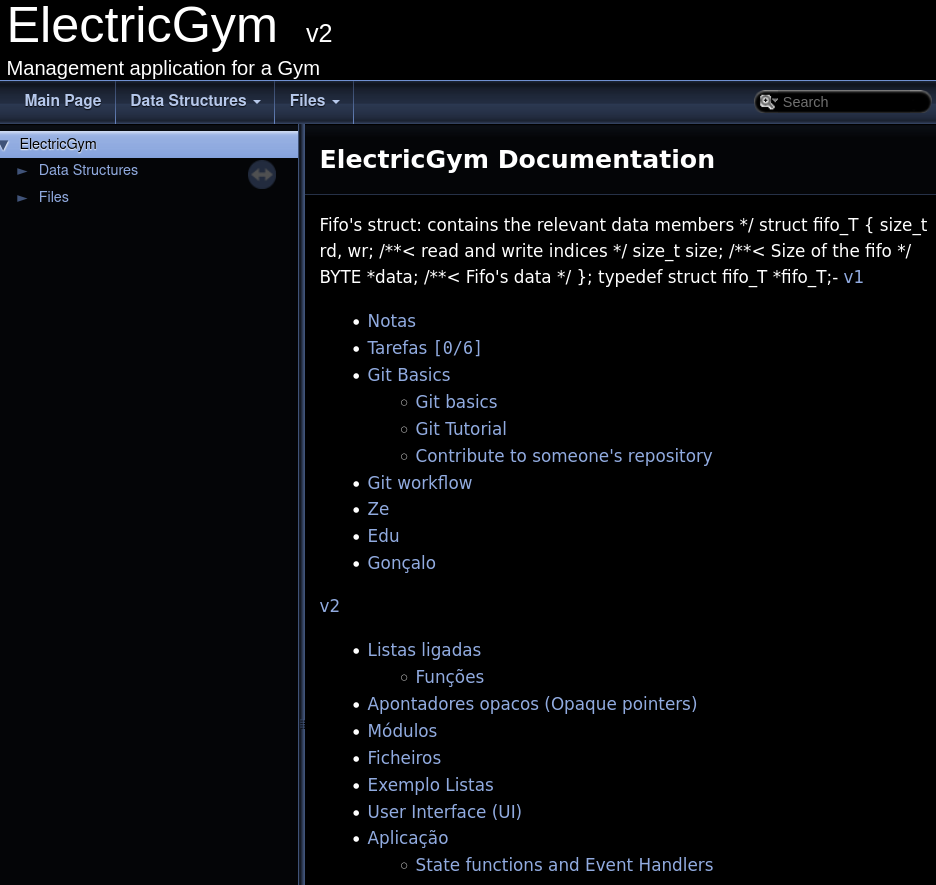
\includegraphics[width=0.8\columnwidth]{./img/doxygen-out1.png}
  \caption{Doxygen output: readme file}%
\label{fig:doxygen-out1}
\end{figure}
%
\begin{figure}[htb!]
\centering
    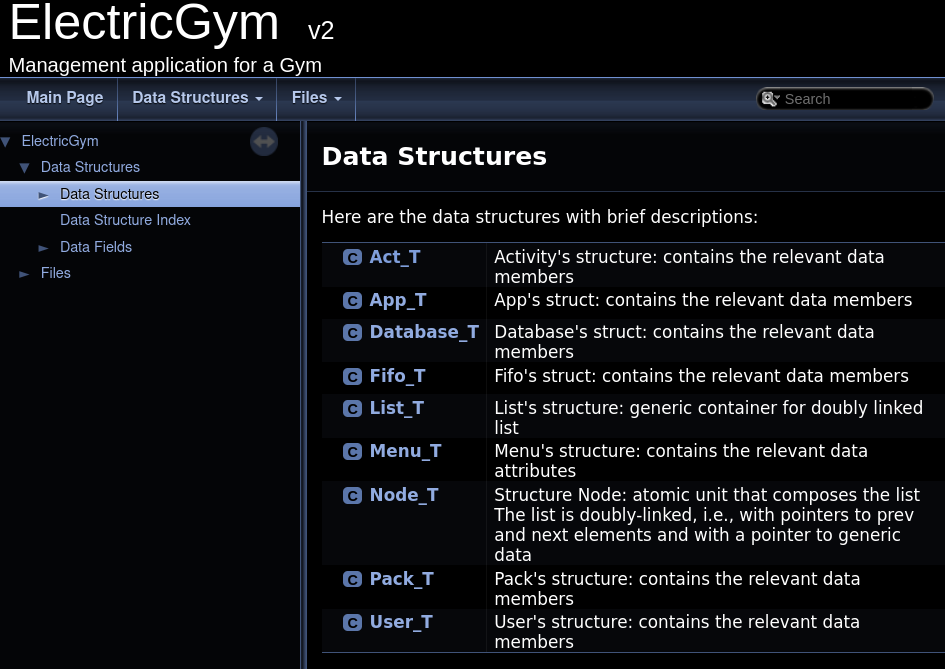
\includegraphics[width=0.8\columnwidth]{./img/doxygen-out2.png}
  \caption{Doxygen output: data structures' overview}%
\label{fig:doxygen-out2}
\end{figure}
%
\begin{figure}[htb!]
\centering
    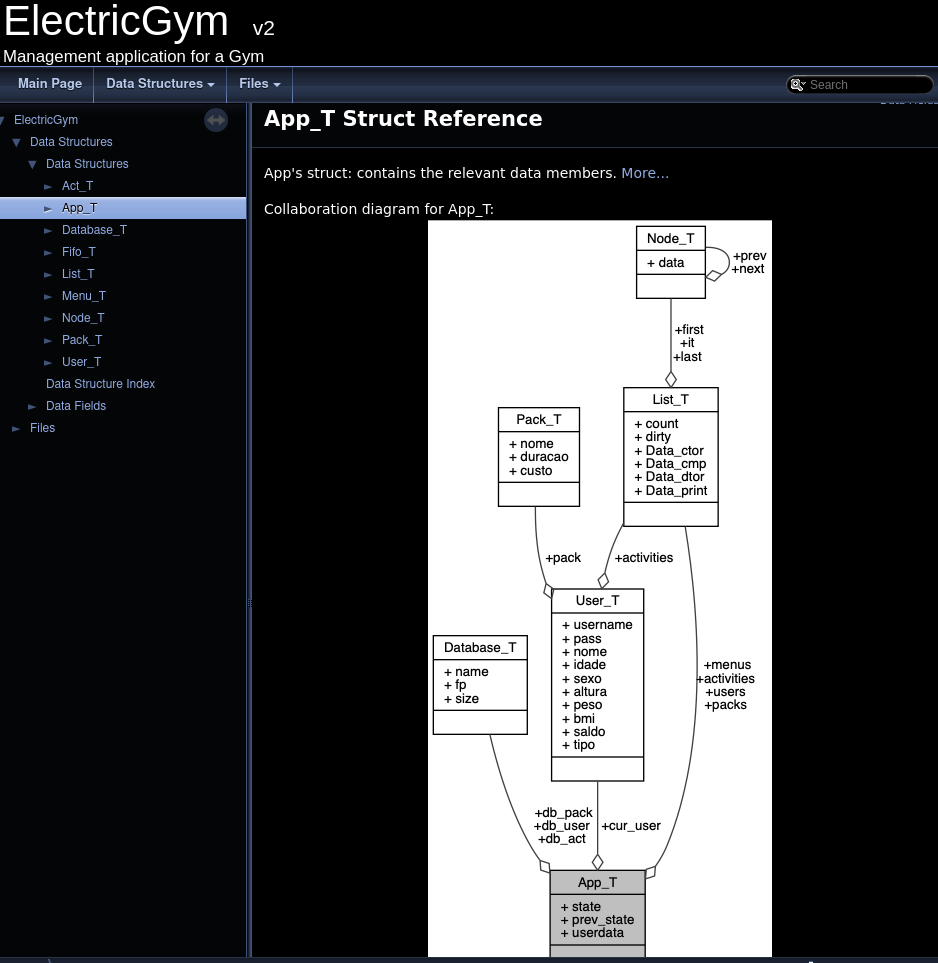
\includegraphics[width=0.8\columnwidth]{./img/doxygen-out3.png}
  \caption{Doxygen output: collaboration graph for a structure}%
\label{fig:doxygen-out3}
\end{figure}
%
\begin{figure}[htb!]
\centering
    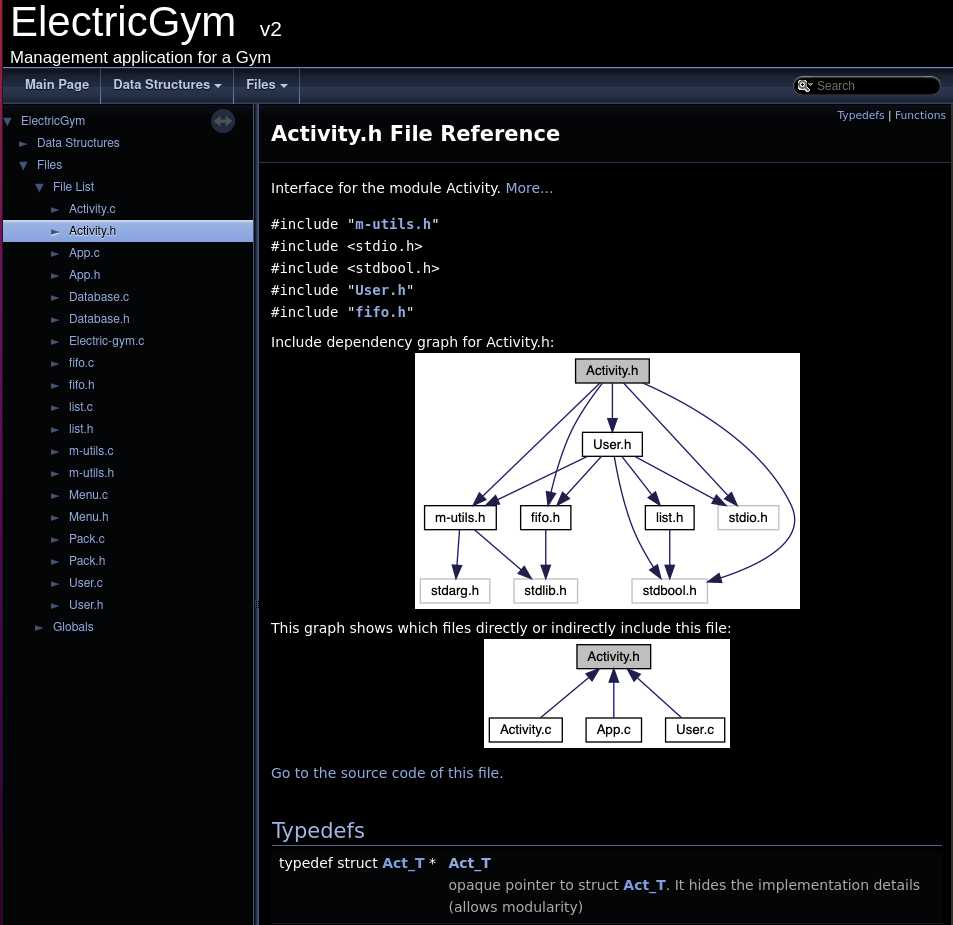
\includegraphics[width=0.8\columnwidth]{./img/doxygen-out4.png}
  \caption{Doxygen output: header file --- dependency graph and \texttt{typedef}}%
\label{fig:doxygen-out4}
\end{figure}
%
\begin{figure}[htb!]
\centering
    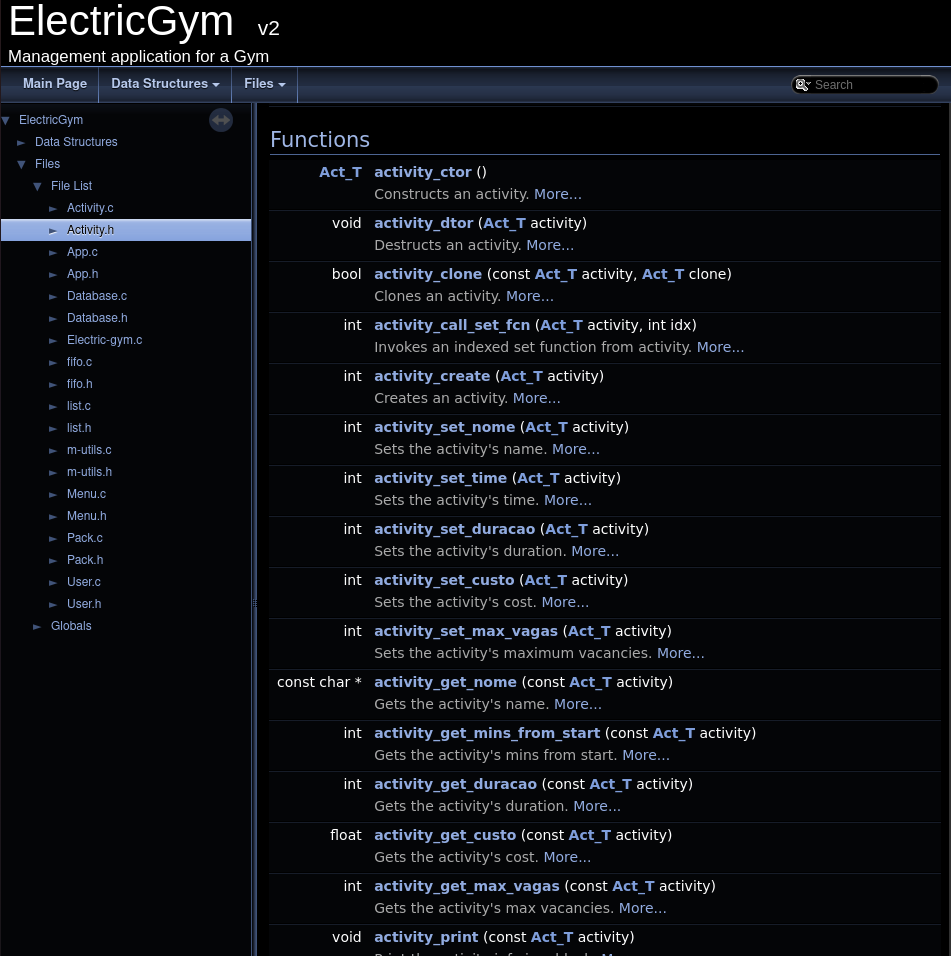
\includegraphics[width=0.8\columnwidth]{./img/doxygen-out5.png}
  \caption{Doxygen output: list of public prototypes for \texttt{Activity}'s module}%
\label{fig:doxygen-out5}
\end{figure}
%
\begin{figure}[htb!]
\centering
    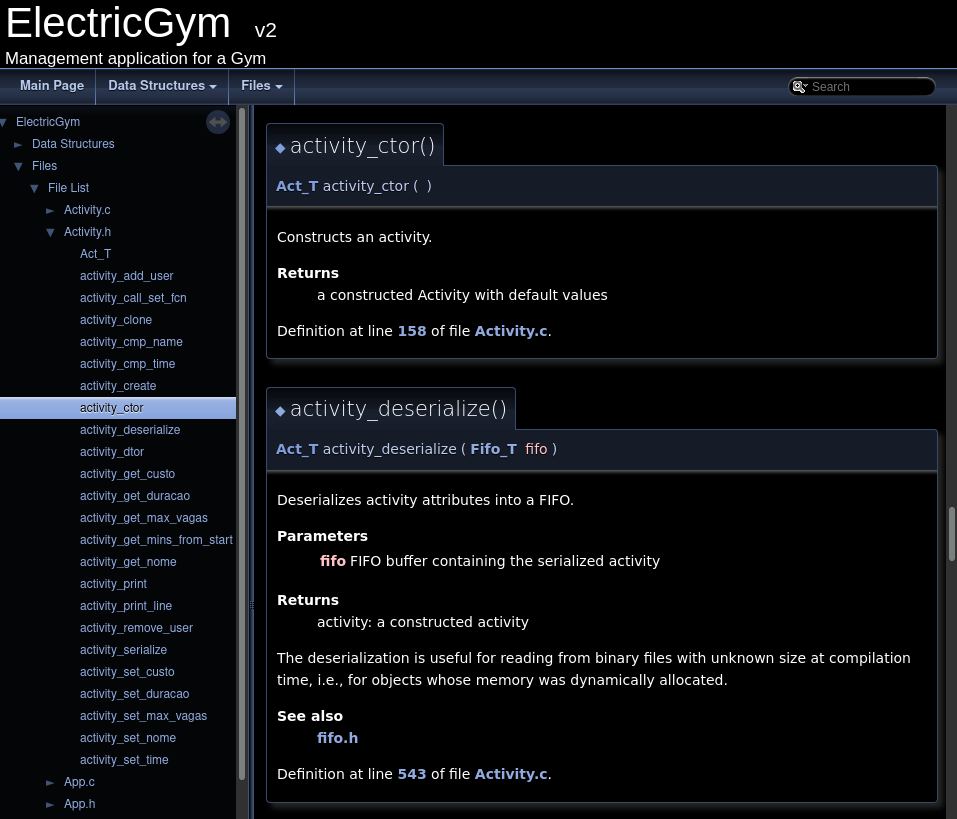
\includegraphics[width=0.8\columnwidth]{./img/doxygen-out6.png}
  \caption{Doxygen output: implementation file --- function details}%
\label{fig:doxygen-out6}
\end{figure}


%%% Local Variables:
%%% mode: latex
%%% TeX-master: "../../../dissertation"
%%% End:
